\chapter{Implementierung}

% Übersicht Komponenten -> Klassen

% Kontrollfluss

% Validierung

%%%%

\begin{figure}[hb] \centering
	\begin{subfigure}[b]{0.4\textwidth}
		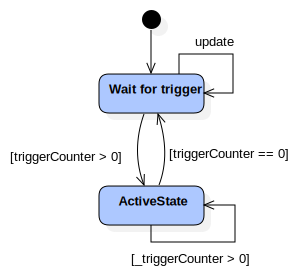
\includegraphics[width=\textwidth]{UML/fallcontroller_simple_loop_statechart.pdf}
		\caption{Einfache Darstellung}
		\label{uml:statechart_simleloop}
	\end{subfigure}\hspace{1cm}
	\begin{subfigure}[b]{0.4\textwidth}
 		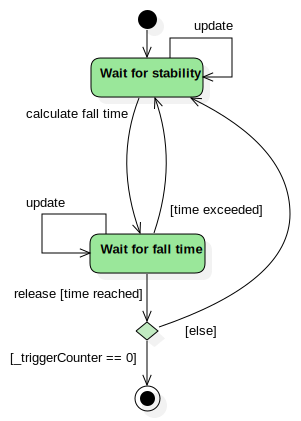
\includegraphics[width=\textwidth]{UML/fallcontroller_active_state_statechart.pdf}
		\caption{Genauere Beschreibung des ActiveStates aus \ref{uml:statechart_simleloop}}
		\label{uml:statechart_activeState}
	\end{subfigure}
	\caption{Beschreibung der Hauptschleife als State-Chart-Diagramm}
	\label{uml:statechart}
\end{figure}

\begin{figure}[hb] \centering
\end{figure}

\begin{figure}[hb] \centering
	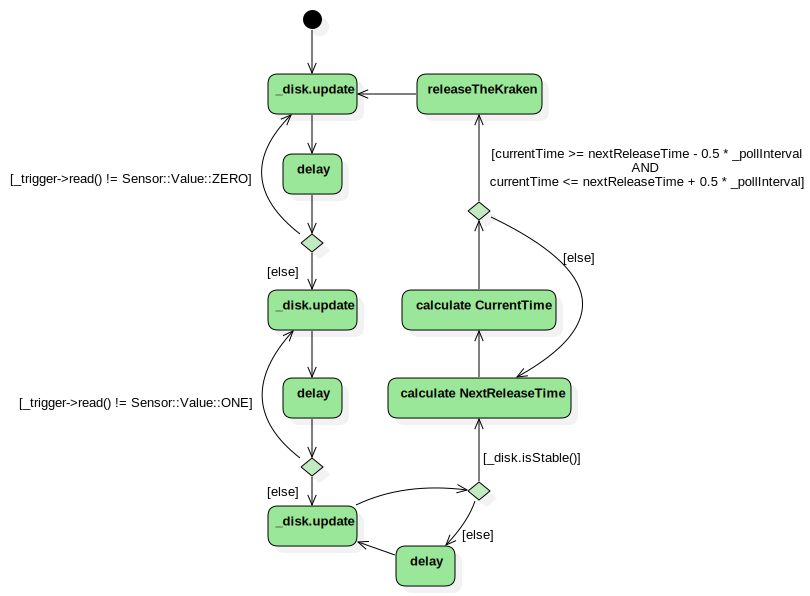
\includegraphics[width=\textwidth]{UML/fallcontroller_loop_activity_diagram.pdf}
	\caption{Genauere Beschreibung der Hauptschleife als Aktivitätsdiagramm}
	\label{uml:activity_diagram}
\end{figure}

\begin{figure}[hb] \centering
	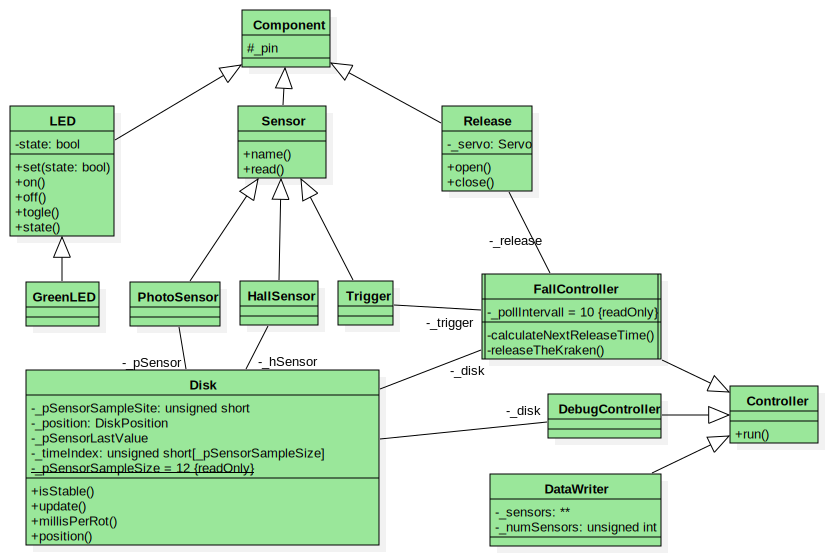
\includegraphics[width=\textwidth]{UML/class_diagram.pdf}
	\caption{Klassendiagramm der Implementierung}
	\label{uml:class_diagram}
\end{figure}
